\bodychapter{Strategy 3: Replication in groups}\label{sec4}
\label{Intro}

 This strategy partitions the processors into $k$ groups
 $G1$,$G2$...$Gk$. The size of each group is equal and have
 $\frac{m}{k}$ processors within each group. For the sake of
 simplicity, we assume that we will only use values of $k$ such that
 $k$ divides $m$. In the first phase, the data of each task is
 replicated on all the processors of one of the $k$ groups,
 i.e. $\forall j, |M_j|= \frac{m}{k}$. In the second phase the tasks
 are scheduled within the group they are assigned to in first phase.
 Figure \ref{fig:Model 3} shows the construction of two phases.
 
 We propose the \textbf{LS-Group} algorithm which is based on Graham's
 List Scheduling algorithm. In phase 1, we use List Scheduling to
 distribute the tasks to the $k$ groups of processors. In phase 2 each
 task is scheduled to a particular processor within the group it was
 allocated in phase 1 using the online List Scheduling algorithm.
 
 \begin{figure*}[htp] 
 \centering
 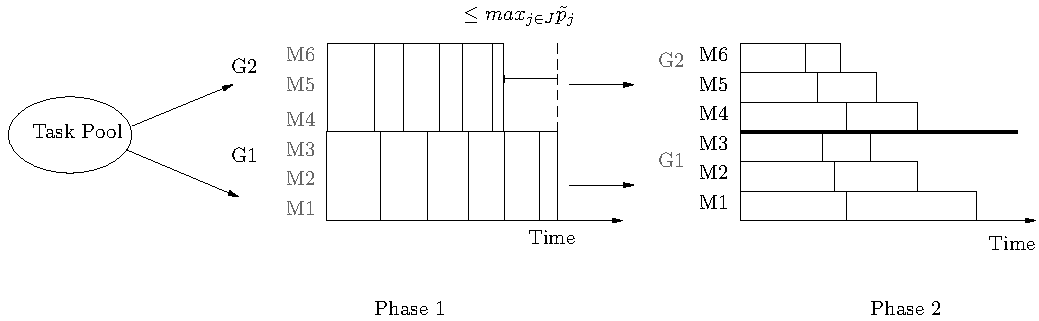
\includegraphics[width=\linewidth]{model3.pdf}
 \caption{An example of replication in groups with $m = 6$, $k = 2$. In
   phase 1, the data of the tasks are assigned to one of the
   groups. Phase 2 schedules each task assigned to a machine within its
   group.}
 \label{fig:Model 3}
 \end{figure*}
 
 \begin{theorem}
   \label{th:strategy3}
   With $k$ groups, the competitive ratio of
   \textbf{LS-Group } is $ \frac{k\alpha^{2}}{\alpha^{2}+k-1} (1+
   {\frac{k-1}{m}} ) + \frac{m-k}{m}$
 \end{theorem}
 \begin{proof} 
   We assume without loss of generality that $ C_{max}$ comes from
   group $G1$. $C_{max}^{*}$ must be greater than the average of the
   loads on the machines.
   \begin{equation}{\nonumber}
     C_{max}^{*} \geq  \frac{\sum_{j \in J}^{}{{p_{j}}}}{m}
   \end{equation}
 
   $\sum_{j \in J }{{p_{j}}}$ can be written as sum of load on $G1$ and
   load on rest of groups.
   \begin{equation}\label{eq11}
     C_{max}^{*} \geq  \frac{\sum_{j \in G1 }^{}{{p_{j}}}+ \sum_{l=2}^{k}\sum_{j \in Gl }^{}{{p_{j}}}}{m}
   \end{equation}
 
   As in phase 1 tasks are allocated to different groups using List
   Scheduling with the estimated processing times of the tasks, the
   (estimated) load difference between any two groups cannot be greater
   than the estimated value of largest task ${max_{j \in J}}{\tilde
     p_{j}}$.  So, for any group $Gl \neq G1$, We have
   \begin{equation}{\nonumber}
 \forall l \in \{2, 3, \dots ,k\}, |\sum_{j \in G1 }^{}{\tilde p_{j}}- \sum_{j \in Gl }^{}{\tilde p_{j}}| \leq {max_{j \in J}}{\tilde p_{j}}
   \end{equation}  
   Adding for all values of $l$ leads to
   \begin{equation}{\nonumber}
     |(k-1)\sum_{j \in G1 }^{}{\tilde p_{j}}- \sum_{l=2}^{k}\sum_{j \in Gl }^{}{\tilde p_{j}}| \leq (k-1) {max_{j \in J}}{\tilde p_{j}}
   \end{equation}
 
   \textbf{Case 1:} If $(k-1)\sum_{j \in G1 }^{}{\tilde p_{j}} >
   \sum_{l=2}^{k}\sum_{j \in Gl }^{}{\tilde p_{j}}$.
   \begin{equation}{\nonumber}
     \sum_{l=2}^{k}\sum_{j \in Gl }^{}{\tilde p_{j}} \geq (k-1) \left( \sum_{j \in G1 }^{}{\tilde p_{j}}- {max_{j \in J}}{\tilde p_{j}} \right)
   \end{equation}
 
   As the actual processing time of the tasks can vary within a factor
   $\alpha$ and $\frac{1}{\alpha}$ of their estimated processing time,
   the following inequality holds
   \begin{equation}{\nonumber}
     \alpha\sum_{l=2}^{k}\sum_{j \in Gl }^{}{{p_{j}}} \geq (k-1) \left( \frac{1}{\alpha}\sum_{j \in G1 }^{}{{p_{j}}}- \alpha {max_{j \in J}}{{p_{j}}} \right)
   \end{equation}
   \begin{equation}\label{eq9}
     \sum_{l=2}^{k}\sum_{j \in Gl }^{}{{p_{j}}} \geq (k-1) \left(\frac{1}{\alpha^{2}}\sum_{j \in G1 }^{}{{p_{j}}}-  {max_{j \in J}}{{p_{j}}} \right)
   \end{equation}
 
   Phase 2 applies List Scheduling in the online mode. We assumed that
   $C_{max}$ comes from $G1$. Using the guarantees of List Scheduling
   we can write,
   \begin{equation}\label{eq10}
     C_{max} \leq \frac{\sum_{j \in G1 }^{}{{p_{j}}}}{m/k} + {\frac{m/k-1}{m/k}} p_{max}
   \end{equation}
   where $p_{max}$ is actual processing time of longest task in $G1$.
 
   From Equation~\ref{eq9} and~\ref{eq11}, we derive
   \begin{equation}{\nonumber}
     C_{max}^{*} \geq  \frac{\sum_{j \in G1 }^{}{{p_{j}}}+ (k-1)\left(\frac{1}{\alpha^{2}}\sum_{j \in G1 }^{}{{p_{j}}}-  {max_{j \in J}}{{p_{j}}}\right)}{m}
   \end{equation}
   \begin{equation}{\nonumber}
     \alpha^{2} (mC_{max}^{*} + (k-1){max_{j \in J}}{{p_{j}}}) \geq  (\alpha^{2} + k-1) \sum_{j \in G1 }^{}{{p_{j}}}  
   \end{equation}
   \begin{equation}\label{eq12}
     \frac{\alpha^{2}}{\alpha^{2}+k-1}\left(m C_{max}^{*}+(k-1) {max_{j \in J}}{{p_{j}}}\right) \geq \sum_{j \in G1 }^{}{{p_{j}}}  
   \end{equation}
   
   Using \ref{eq10} and \ref{eq12}, We have
   \begin{align}{\nonumber}
     C_{max} \leq \frac{k\alpha^{2}}{\alpha^{2}+k-1}\left( C_{max}^{*}+\frac{k-1}{m} {max_{j \in J}}{{p_{j}}}\right)\\
     + {\frac{m/k-1}{m/k}} p_{max} \nonumber
   \end{align}
   
   As $C_{max}^{*}\geq {{max_{j \in J}}{p_{j}}}\geq p_{max}$, we have
   \begin{align}{\nonumber}
     C_{max} \leq \frac{k\alpha^{2}}{\alpha^{2}+k-1}\left( C_{max}^{*}+ {\frac{k-1}{m}}{C_{max}^{*}}\right)\\
     + {\frac{m-k}{m}} C_{max}^{*} \nonumber
   \end{align}    
   
   So, in Case 1 the algorithm has a competitive ratio of,
   \begin{equation}{\nonumber}
     \frac{C_{max}}{C_{max}^{*}} \leq \frac{k\alpha^{2}}{\alpha^{2}+k-1}\left( 1+ {\frac{k-1}{m}} \right) + {\frac{m-k}{m}} \end{equation}\\
   
   \textbf{Case 2:} If $(k-1)\sum_{j \in G1 }^{}{\tilde p_{j}} \leq \sum_{l=2}^{k}\sum_{j \in Gl }^{}{\tilde p_{j}}$. \\
   
   Since the processing times of the tasks can vary within a factor
   $\alpha$ and $\frac{1}{\alpha}$ of their estimated values, the
   expression for case 2 can be written as
   \begin{equation}{\nonumber}
     \sum_{l=2}^{k}\sum_{j \in Gl }^{}{ p_{j}} \geq \frac{1}{\alpha^2} (k-1)\sum_{j \in G1 }^{}{ p_{j}}
   \end{equation}
   
   Putting this value in Equation~\ref{eq11}, we have
   \begin{equation}\label{eq13}
     C_{max}^{*} \geq \frac{\alpha^2+k-1}{m\alpha^2}\sum_{j \in G1 }^{}{ p_{j}}
   \end{equation}
   Using Equations~\ref{eq10} and~\ref{eq13}, and as $C_{max}^{*} \geq p_{max}$, we have
   \begin{equation}{\nonumber}
     C_{max} \leq \frac{k\alpha^2}{\alpha^2+k-1}C_{max}^{*}+\frac{m-k}{m}C_{max}^{*}
   \end{equation}
   
   So, in case 2 the algorithm has a competitive ratio of
   $\frac{k\alpha^2}{\alpha^2+k-1}+\frac{m-k}{m}$.
 
   Clearly, the algorithm has a worst competitive ratio in case 1.  So,
   the algorithm has a competitive approximation ratio of
   $\frac{C_{max}}{C_{max}^{*}} \leq \frac{k\alpha^{2}}{\alpha^{2}+k-1}
   \left( 1+ {\frac{k-1}{m}} \right) + {\frac{m-k}{m}}$.
 \end{proof}
 
 % \begin{corollary}
 %   When there are $2$  groups, the competitive ratio is $ 1+
 %   \frac{2}{1+\alpha^{2}} (\alpha^2-\frac{1}{m})$.
 % \end{corollary}
 
 \textbf{LS-Group} uses List Scheduling in both its phases. A LPT-based
 algorithm may have better guarantee. But without performing any
 replication, {\em i.e.} when $k=m$, the \textbf{LS-Group} algorithm
 has a competitive ratio almost equal to \textbf{LPT-No choice}'s when
 the number of machines $m$ is large and the value of $\alpha$ is
 within practical range. This indicates an LPT-based algorithm for
 strategy 3 would likely not have a much more interesting guarantee.